\begin{tikzpicture}

\GraphInit[vstyle=Classic]

\Vertex[Lpos=-90, x=0, y=0, L=$p_{1}$]{p1};
\Vertex[Lpos=-90, x=2, y=0, L=$p_{2}$]{p2};
\Vertex[Lpos=-90, x=4, y=0, L=$p_{3}$]{p3};
\Vertex[Lpos=-90, x=6, y=0, L=$p_{4}$]{p4};
\Vertex[Lpos=-90, x=8, y=0, L=$p_{s - 1}$]{psm1};
\Vertex[Lpos=-90, x=10, y=0, L=$p_{s}$]{ps};

\Edge[style ={-},label={$a_{1}$},labelstyle={above}]({p1})({p2})
\Edge[style ={draw=none},label={$(a_{2})$},labelstyle={below}]({p1})({p2})
\Edge[style ={-},label={$a_{2}$},labelstyle={above}]({p2})({p3})
\Edge[style ={draw=none},label={$(a_{3})$},labelstyle={below}]({p2})({p3})
\Edge[style ={-},label={$a_{3}$},labelstyle={above}]({p3})({p4})
\Edge[style ={draw=none},label={$(a_{4})$},labelstyle={below}]({p3})({p4})
\Edge[style ={-, dashed},labelstyle={above}]({p4})({psm1})
\Edge[style ={-},label={$a_{s - 1}$},labelstyle={above}]({psm1})({ps})
\Edge[style ={draw=none},label={$(a_{s})$},labelstyle={below}]({psm1})({ps})

\end{tikzpicture}
